\subsection*{b)}
Erläutern Sie kurz, wie im UML‐Metamodell Modellierungskonzepte erklärt werden.


\section*{Antwort}
Das UML-Metamodell regelt, in welchem Zusammenhang \textbf{UML-Modellierungskonzepte} in Modellen auftreten dürfen, und welche \textit{Eigenschaften} und \textit{Beziehungen} zwischen den Modellelementen erlaubt sind (vgl.~\cite[81]{Buh09}).\\
Das UML-Metamodell wird auf Basis des Metamodells der \textbf{Meta Object Facility} (\textit{MOF}\footnote{
\url{https://www.omg.org/mof}, abgerufen 15.05.2024
}) definiert (vgl.~\cite[5]{Buh09}).

\noindent
Ein \textbf{Modellelement} ist hierbei eine \textit{Instanz} eines bestimmten UML-Modellierungskonzeptes: Modellelemente werden von Benutzern erstellt (s. Abbildung~\ref{fig:metamodel}).\\

\noindent
Die im Metamodell verwendeten Erklärungen basieren auf einer abstrakten Syntax, die mittels einer Untermenge der UML (\textbf{Klassendiagramme}) beschrieben wird.\\

\noindent
Die Semantik der Modellierungskonzepte wird textlich beschrieben, die Syntax wird über die \textbf{OCL} formalisiert.

\begin{figure}
    \centering
    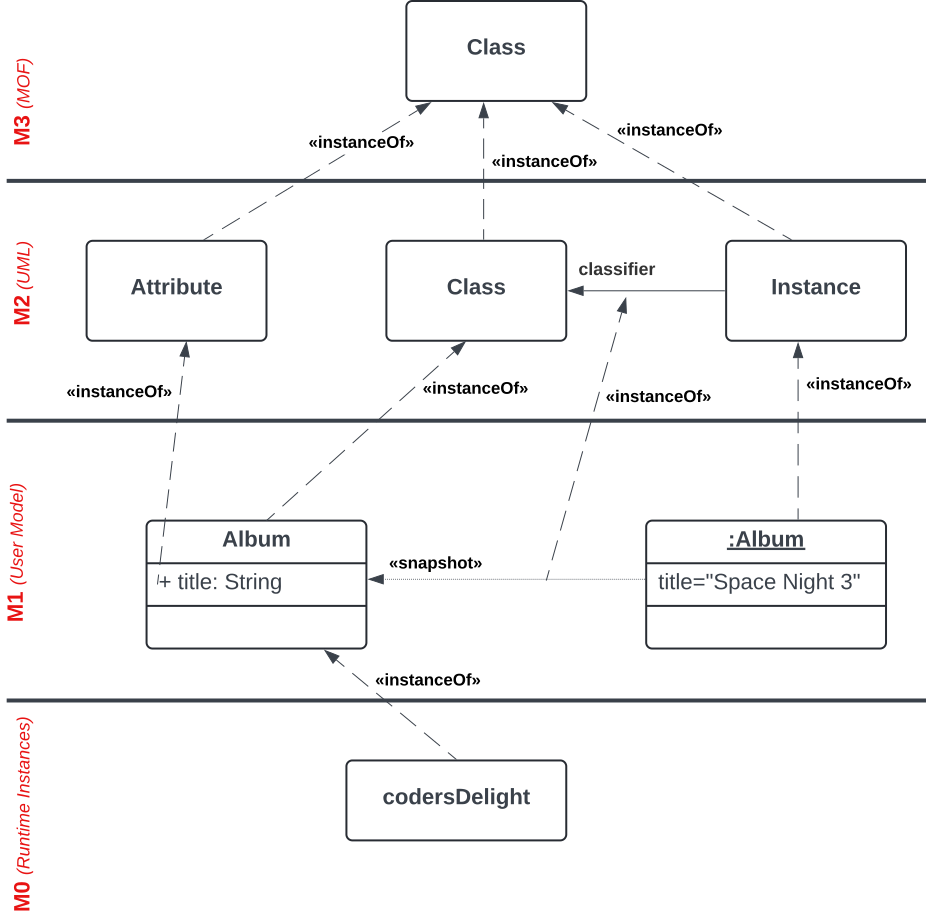
\includegraphics[scale=0.4]{chapters/aufgabe 1/img/metamodel}
    \caption{Beispiel für die verschiedenen Schichten der Metamodell Hierarchie. (Quelle: in Anlehnung an S. 20, Figure 7.8, \url{https://www.omg.org/spec/UML/2.4.1/Infrastructure/PDF}, abgerufen 15.05.2024}
    \label{fig:metamodel}
\end{figure}